\chapter{\noun{Use cases}   }
In his chapter we present sequence diagram of the actions performed in the range of Pharmacy Module. Each step is detailed described. Not all actions are strongly required - sometimes it should depend on the security level requirement and budget possibilities. 

The first step is communication initialization. Actions performed in this step by the system elements are presented in the figure \ref{fig:s_q_step_1}
\begin{figure}
    \centering
    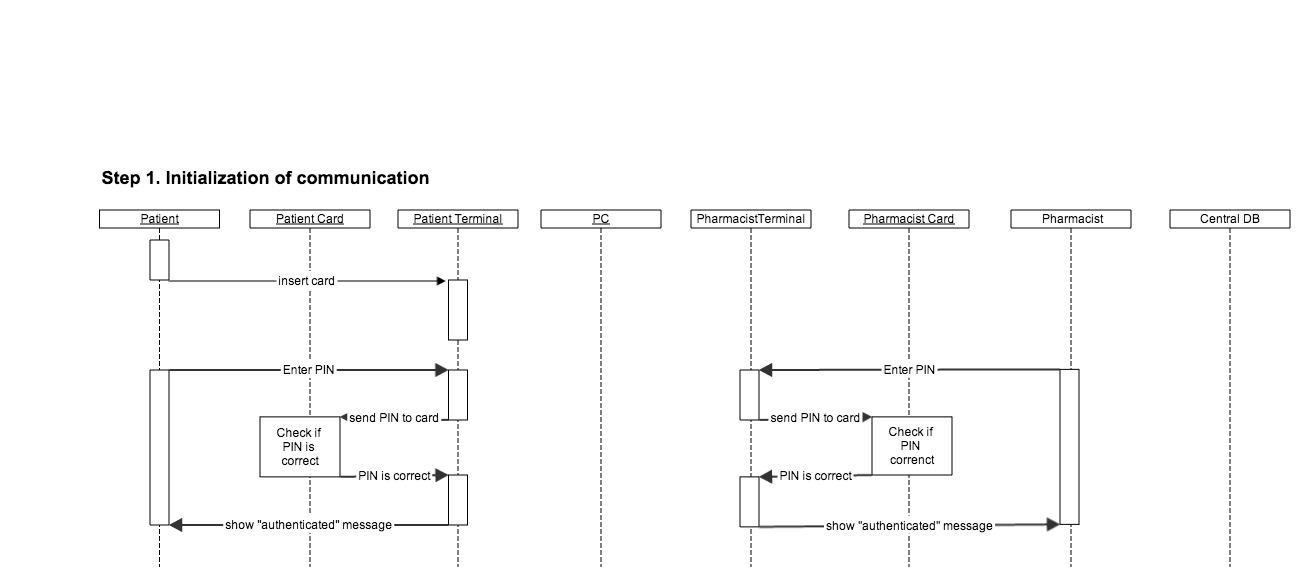
\includegraphics[width=1\textwidth]{s_d_1.png}
    \caption{General use case}
    \label{fig:s_q_step_1}
\end{figure} 
